\begin{atiTask}[
  title = Spezielle Vektorfelder
]

\begin{atiSubtasks}
\item Es sei $\Phi$ ein skalares Feld und $\vec{A}$ ein Vektorfeld. Beweisen Sie die Beziehung
\[
\divergence (\Phi \vec{A})=\vec{A}\cdot\gradient \Phi+\Phi\cdot \divergence \vec{A}.
\]
\item Spezialisieren Sie das Resultat von (a) für den Fall $\vec{A}=\gradient \Phi$.
\item Das skalare Feld $\Phi$ erfülle nun die Bedingungen $\Phi=0$ auf $S$ und $\Delta \Phi=0$ in $V$, worin $\Delta$ den \textsc{Laplace}-Operator und $S$ die Fläche bezeichnet, die das Volumen $V$ umgibt. Zeigen Sie, dass $\phi=0$ in $V$ gilt.
%\item In diesem Aufgabenteil sei $\vec{A}=\vec{c}$ ein konstanter Vektor. Weisen Sie die Gültigkeit der Beziehung
%\[
%\iiint\limits_{V}\gradient \Phi\;\mathrm{d}V=\oiint\limits_{S}\Phi\;\mathrm{d} \vec{f}
%\]
%nach.
\end{atiSubtasks}


\end{atiTask}

\begin{atiSolution}
	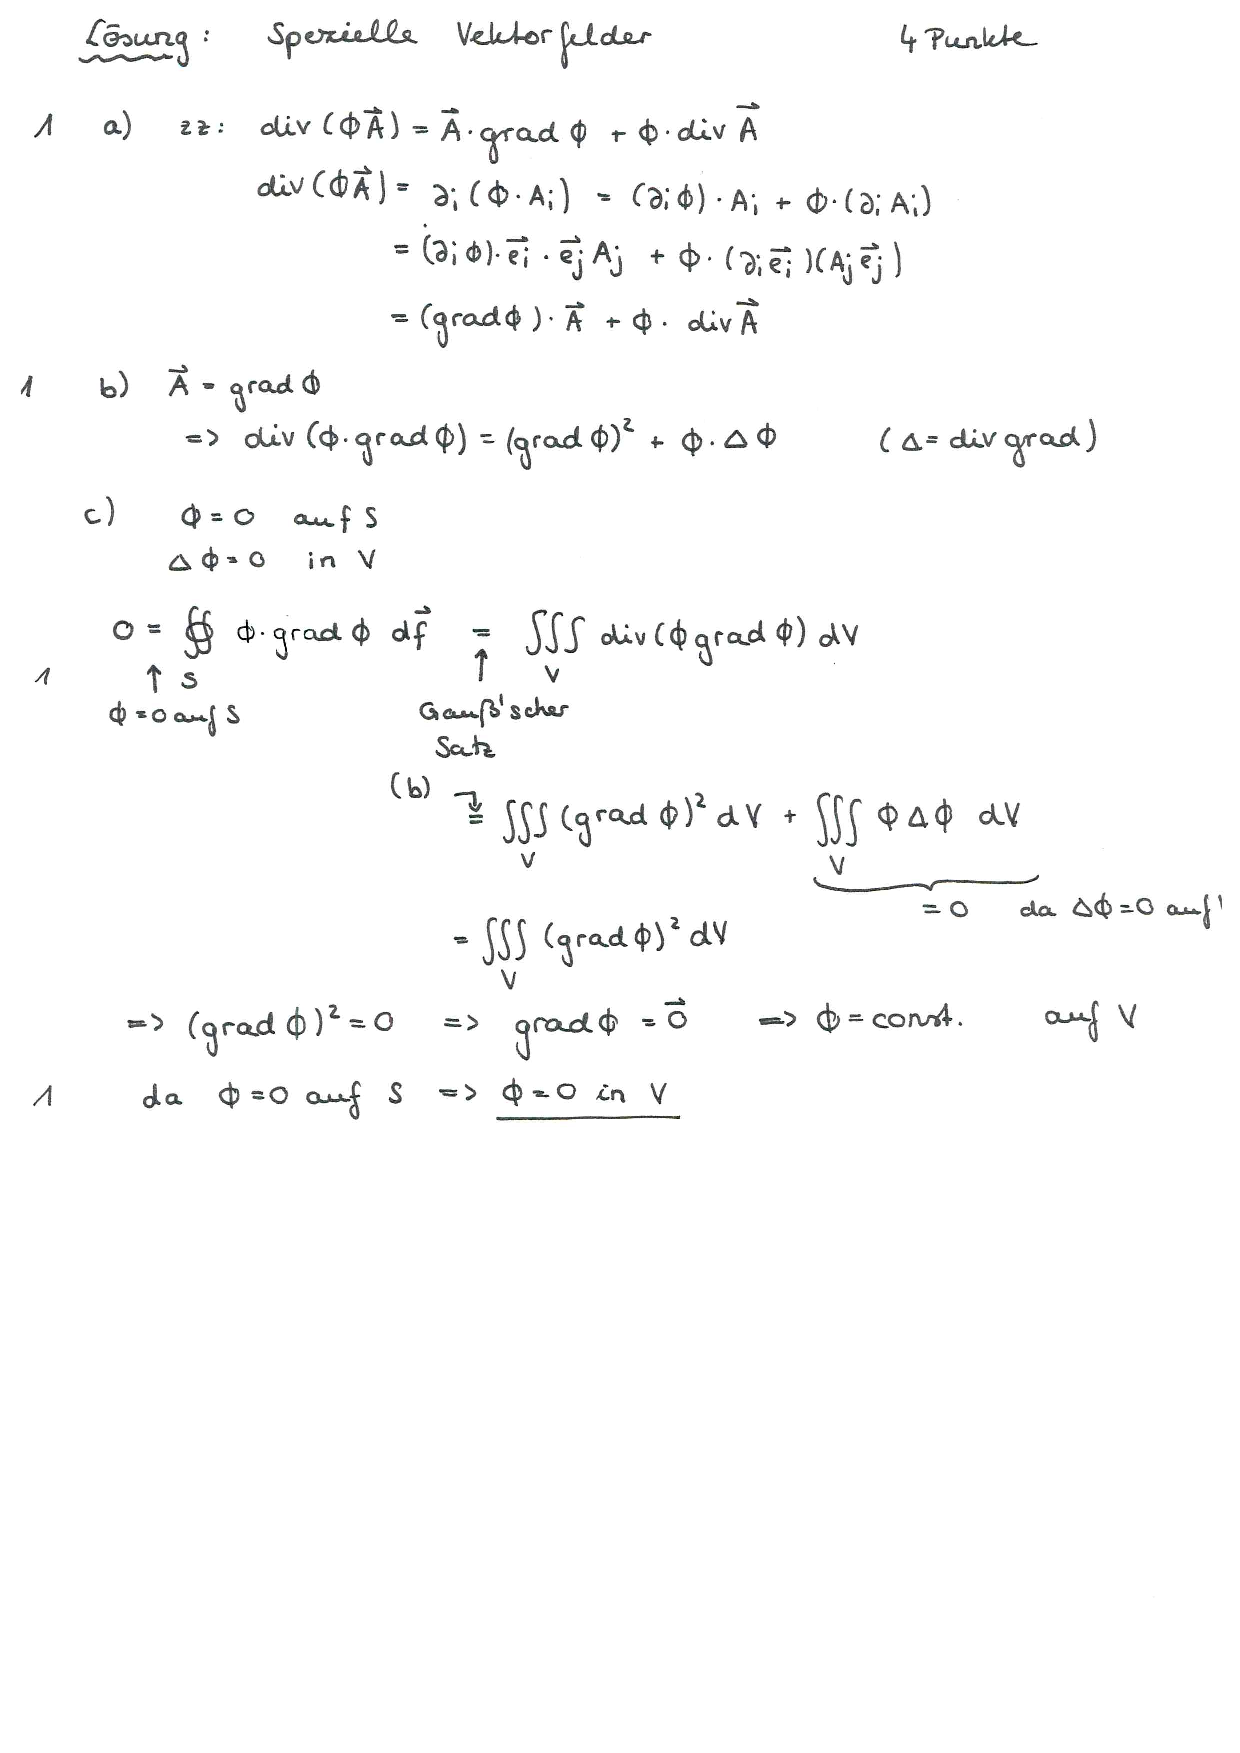
\includepdf[pages=-]{solution-index_iii.pdf}
\end{atiSolution}
